\chapter{Results}

\begin{center}
    \textit{This chapter presents the outcomes of the project, including the functionality and performance of the developed application. It highlights the achieved results in relation to the project goals and requirements.}
\end{center}

\section{Overview of Delivered Product}
The delivered product refers to the final version of the application submitted at the conclusion of this Bachelor’s thesis. The application was developed at the request of the product owner and based on the requirements provided. The initial description served as a general concept rather than a detailed specification, which meant that decisions regarding design, architecture, and technology were left to the development team. Throughout the development process, ideas and design choices were discussed with the product owner and approved during regular meetings. \\

The application was developed as an open-source project with the intention that the code can be reused, maintained, and extended by others. All components are built using open and freely available technologies, ensuring that the system can be installed on local hardware without the need for licensed software or cloud-based services. This aligns with the requirement that all processing should be performed locally, using common hardware such as a webcam connected to a local machine running either Windows or Ubuntu. \\

The project follows clear coding standards and development best practices, making the code easy to understand and modify. All functionality is well documented, enabling future developers to build upon the existing solution. For example, to support new chess variants, integrate additional hardware, or improve the recognition models. To support future development and accessibility, the source code is published in a public Git repository without restrictions on reuse or adaptation. \\

The application itself is a local, camera-based system for digitalizing over-the-board chess games in real time. It detects piece movements on a physical chessboard using image recognition and converts the game into a PGN file, which can be viewed or analyzed digitally. The system operates entirely on local hardware, with a front-end interface that allows users to follow games live and a back-end that manages board recognition and game logic. The application is designed to be low-cost, open-source, and easy to maintain, with extensibility in mind for future features.

\section{Functional Results}
The application consists of three main components: machine learning, WebSocket communication, and the front-end interface. The back-end handles image recognition and game logic, using a machine learning model to detect board states. It communicates with the front-end through a WebSocket connection. The front-end is responsible for presenting this information to the user in real time. The cameras is connected with a USB-hub, where multiple cameras can be attached to the same computer. 

\subsection{Machine Learning}
To be completed.

\subsection{API}
To enable real-time updates and improve the responsiveness of the front-end interface, the application uses a WebSocket connection between the back-end and the front-end. This method was suggested by the product owner and was also approved by the supervisor. This communication channel is used for transmitting move data as it is detected by the board recognition system. Unlike traditional HTTP requests, which operate on a request-response basis, WebSocket allows for continuous, two-way communication between the server and the client. \\

Once the application initiates a connection, the WebSocket remains open throughout the session. As new moves are identified on the physical board, the back-end sends the corresponding move data as messages through the WebSocket. These messages are then received by the front-end, which updates the displayed move list and board state in real time. This provides a seamless viewing experience for users following live games. \\

The WebSocket server also handles specific command messages. For example, when the server sends a message labeled "RESET," the front-end clears the current move list, typically indicating the start of a new game. A message labeled "INVALID" is used to signal an unrecognized or incorrect move and does not trigger any front-end changes. All other messages are assumed to be valid algebraic notation representing chess moves and are appended to the game history displayed to the user. \\

The WebSocket functionality is encapsulated in a custom React hook on the front-end, which manages the connection lifecycle and state updates. This abstraction simplifies integration into the user interface and ensures that resources are properly cleaned up when the component is unmounted. Overall, the use of WebSocket communication is a key component in delivering a responsive and live experience, particularly for tournaments and public displays where move-by-move tracking is essential.

\subsection{Frontend}
The front-end of the application serves as the user interface. It includes a control panel for tournament organizers and a web application for spectators. The application's main responsibility is to visualize the chessboard and display ongoing moves. The front-end communicates with the back-end via WebSocket to ensure real-time updates and interactivity. \\

The \textbf{control panel} is an administrative tool accessible only to the tournament organizers. It functions as a standalone dashboard application and is available exclusively on the computer that starts the application, as shown in Figure~\ref{fig:control-panel}. This setup ensures that spectators visiting the website cannot access the control panel. \\

\begin{figure}[h!] \centering 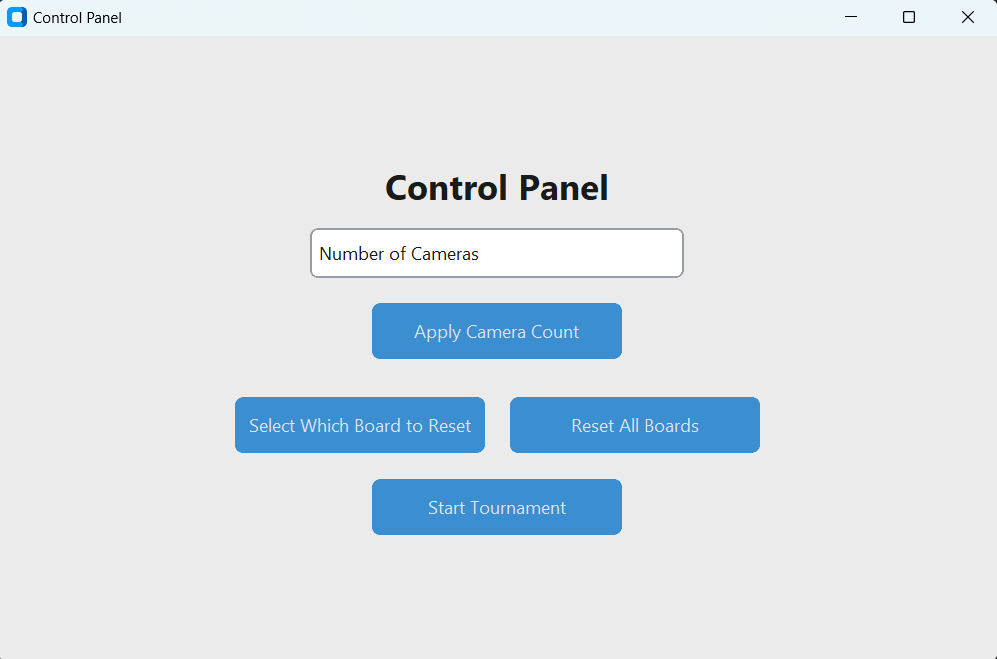
\includegraphics[width=0.75\linewidth]{figures/results/frontend/controlpanel.png} \caption[Control panel for tournament organizers]{The control panel used by the tournament organizers.}\label{fig:control-panel} \end{figure}

Before the tournament begins, the organizer must start the application and configure it using the control panel. This includes specifying the number of cameras to be used, allowing the application to connect to the appropriate number of video feeds. When the number of selected cameras is connecting, a progress bar is visible for the user, as shown in Figure~\ref{fig:control-panel-camera} Once the connections are established, the tournament can be started by pressing the "Start Tournament" button. \\
 
\begin{figure}[h!] \centering 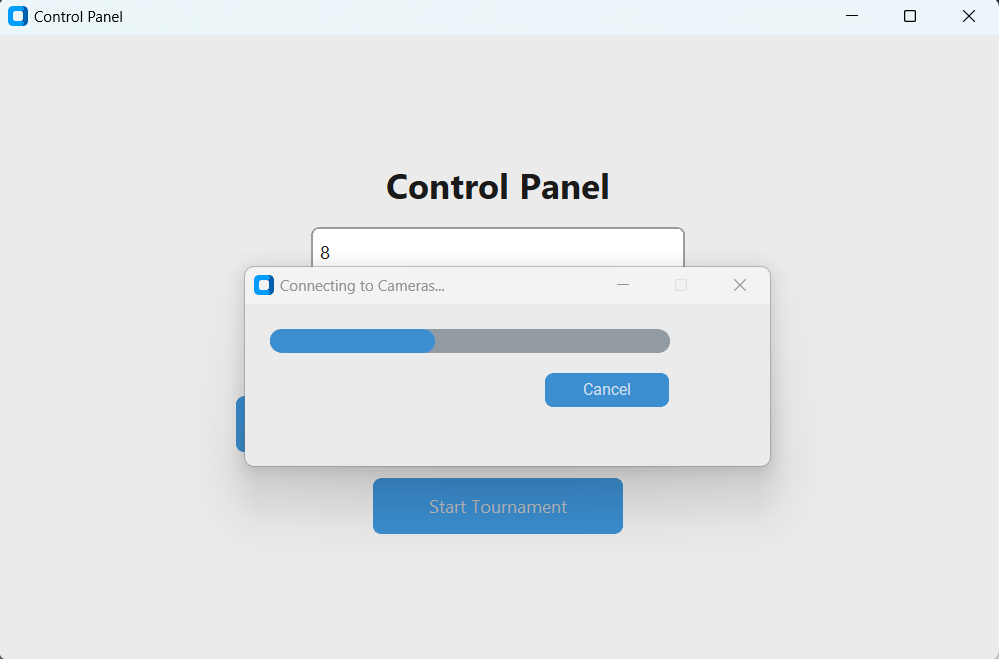
\includegraphics[width=0.75\linewidth]{figures/results/frontend/controlpanel-camera.png} \caption[Progress bar for camera connections]{A progress bar representing the status of connecting cameras}\label{fig:control-panel-camera} \end{figure}

The control panel also provides functionality for resetting individual boards or all boards simultaneously. When a tournament round is finished, the organizers must reset all boards before the next round can begin. By pressing the "Reset All Boards" button, they can reset all connected boards at once. In some scenarios, it may be necessary to reset a single board. In such cases, the organizers can use the "Select Which Board to Reset" feature, as shown in Figure~\ref{fig:control-panel-reset-boards}.\

\begin{figure}[h!] \centering 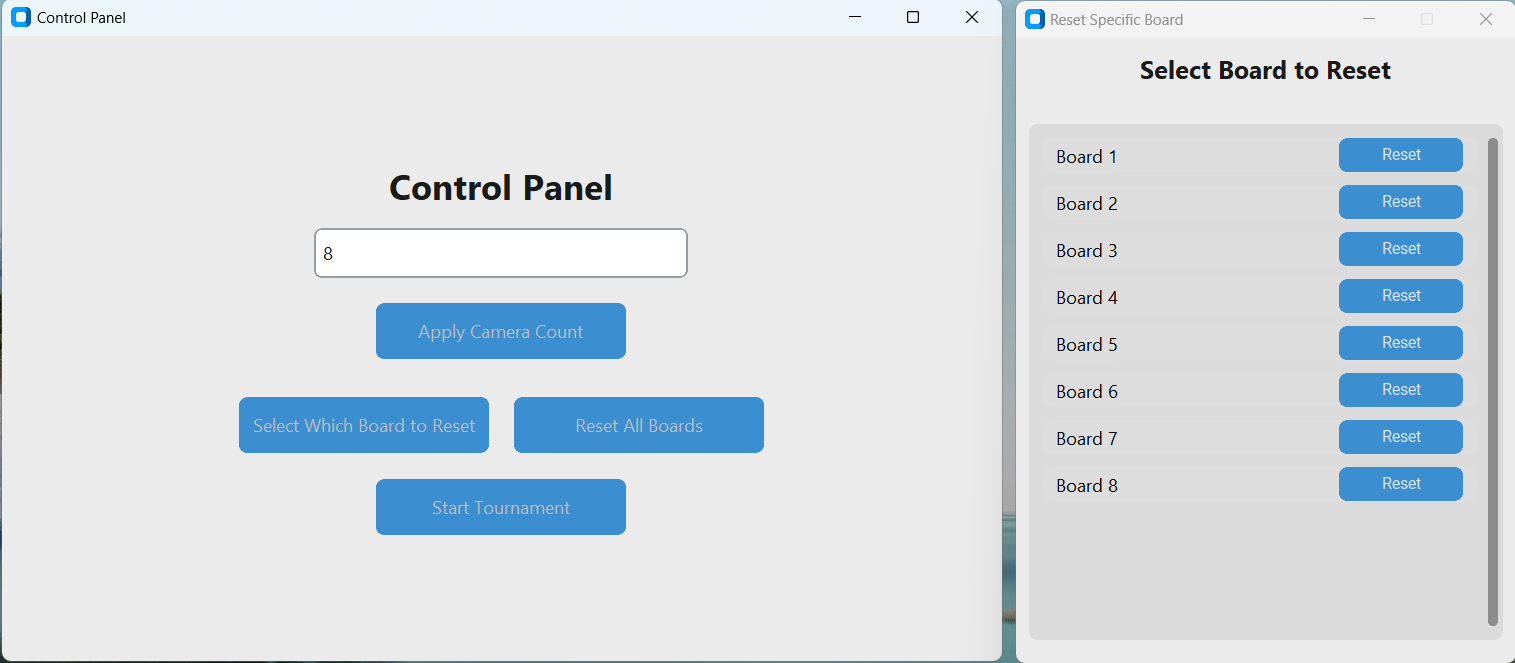
\includegraphics[width=0.75\linewidth]{figures/results/frontend/controlpanel-reset-boards.png} \caption[Panel to reset a single board]{The panel to select which board to be reset}\label{fig:control-panel-reset-boards} \end{figure}

